%%%%%%%%%%%%%%%%%%%%%%%%%%%%%%%%%%%%%%%%%%%%%%%
%%% Template for lab reports used at STIMA
%%%%%%%%%%%%%%%%%%%%%%%%%%%%%%%%%%%%%%%%%%%%%%%

%%%%%%%%%%%%%%%%%%%%%%%%%%%%%% Sets the document class for t hyhe document
% Openany is added to remove the book style of starting every new chapter on an odd page (not needed for reports)
\documentclass[10pt,swedish, openany]{book}

%%%%%%%%%%%%%%%%%%%%%%%%%%%%%% Loading packages that alter the style
\usepackage[]{graphicx}
\usepackage[]{color}
\usepackage{alltt}
\usepackage[T1]{fontenc}
\usepackage[utf8]{inputenc}
\usepackage{listings}
\usepackage{xcolor}
\usepackage{mathtools}



%New colors defined below
\definecolor{codegreen}{rgb}{0,0.6,0}
\definecolor{codegray}{rgb}{0.5,0.5,0.5}
\definecolor{codepurple}{rgb}{0.58,0,0.82}
\definecolor{backcolour}{rgb}{0.95,0.95,0.92}

%Code listing style named "mystyle"
\lstdefinestyle{mystyle}{
  backgroundcolor=\color{backcolour}, commentstyle=\color{codegreen},
  keywordstyle=\color{magenta},
  numberstyle=\tiny\color{codegray},
  stringstyle=\color{codepurple},
  basicstyle=\ttfamily\footnotesize,
  breakatwhitespace=false,         
  breaklines=true,                 
  captionpos=b,                    
  keepspaces=true,                 
  numbers=left,                    
  numbersep=5pt,                  
  showspaces=false,                
  showstringspaces=false,
  showtabs=false,                  
  tabsize=2
}
\setcounter{secnumdepth}{3}
\setcounter{tocdepth}{3}
\setlength{\parskip}{\smallskipamount}
\setlength{\parindent}{0pt}


% Set page margins
\usepackage[top=100pt,bottom=100pt,left=68pt,right=66pt]{geometry}

% Package used for placeholder text
\usepackage{lipsum}

% Prevents LaTeX from filling out a page to the bottom
\raggedbottom

% Adding both languages, Spanish and English, so they can be used intermittently in for example abstracts.
\usepackage[spanish, english]{babel}

% All page numbers positioned at the bottom of the page
\usepackage{fancyhdr}
\fancyhf{} % clear all header and footers
\fancyfoot[C]{\thepage}
\renewcommand{\headrulewidth}{0pt} % remove the header rule
\pagestyle{fancy}

% Changes the style of chapter headings
\usepackage{titlesec}
\titleformat{\chapter}
   {\normalfont\LARGE\bfseries}{\thechapter.}{1em}{}
% Change distance between chapter header and text
\titlespacing{\chapter}{0pt}{50pt}{2\baselineskip}

% Adds table captions above the table per default
\usepackage{float}
\floatstyle{plaintop}
\restylefloat{table}

% Adds space between caption and table
\usepackage[tableposition=top]{caption}

% Adds hyperlinks to references and ToC
\usepackage{hyperref}
\hypersetup{hidelinks,linkcolor = black} % Changes the link color to black and hides the hideous red border that usually is created

% If multiple images are to be added, a folder (path) with all the images can be added here 
\graphicspath{ {images/} }

% Separates the first part of the report/thesis in Roman numerals
\frontmatter

\lstset{style=mystyle}

%%%%%%%%%%%%%%%%%%%%%%%%%%%%%% Starts the document
\begin{document}

%%% Selects the language to be used for the first couple of pages
\selectlanguage{spanish}

%%%%% Adds the title page
\begin{titlepage}
	\clearpage\thispagestyle{empty}
	\centering
	\vspace{2cm}

	% Titles
	{\large Procesamiento de Datos a Gran Escala \par}
	\vspace{4cm}
	{\Huge \textbf{Práctica 1}} \\
	\vspace{1cm}
	{\large \textbf{Hadoop y Tutorial de Spark} \\} %\\
	%{\large \textit{Cifrado. Dando cambio. Subsecuencias. BST óptimos.}} \par}
	\vspace{4cm}
	{\normalsize María Barroso Honrubia \\ % \\ specifies a new line
	             Gloria del Valle Cano \par}
	              \href{mailto:maria.barrosoh@estudiante.uam.es}{maria.barrosoh@estudiante.uam.es} \&
	              \href{mailto:gloria.valle@estudiante.uam.es}{gloria.valle@estudiante.uam.es} \\
	\vspace{2cm}

    
\includegraphics[scale=0.28]{logoEPSofi.jpg}
    
    \vspace{1.7cm}
    
	% Information about the University
	{\normalsize Máster en Ciencia de Datos \\ 
		Escuela Politécnica Superior \\
		Universidad Autónoma de Madrid \par}
		
	% Set the date
	\date{today}
	\vspace{2cm}
	
	\pagebreak

\end{titlepage}

% Adds a table of contents
\tableofcontents{}

\clearpage


\clearpage


%%%%%%%%%%%%%%%%%%%%%%%%%%%%%%%%%%%%%%%%%%%%%%%%%%%%%%%%%%%%%%%%%%%%%%%%%%%%%%%%%%%%%%%%%%%%
%%%%%%%%%%%% The rows above should not be changed except for the title page information
%%%%%%%%%%%%%%%%%%%%%%%%%%%%%%%%%%%%%%%%%%%%%%%%%%%%%%%%%%%%%%%%%%%%%%%%%%%%%%%%%%%%%%%%%%%%
%%%%% Text body starts here!
\mainmatter




\chapter{Hadoop}

En la máquina virtual proporcionada con la versión de Java 1.7 compatible con Hadoop 2.8 y desde el usuario \texttt{root} se descomprime Hadoop y se mueve a \texttt{/opt/}. Se crea un enlace a Hadoop utilizando el comando 
\begin{lstlisting}[language=, caption=]
ln -s hadoop-2.8.1 hadoop
\end{lstlisting}
y se edita el fichero \texttt{etc/hadoop/hadoop-env.sh} para exportar la variable \texttt{JAVA\_HOME} con la versión de Java correcta. A continuación se configura \texttt{ssh} para funcionar sin contraseña para conexiones \textit{localhost}:
  \begin{lstlisting}[language=, caption=]
ssh-keygen 
ssh-copy-id localhost
\end{lstlisting}

Finalmente se configura Hadoop HDFS modificando los ficheros \texttt{ /opt/hadoop/etc/hadoop/core-site.xml} y \texttt{ /opt/hadoop/etc/hadoop/hdfs-site.xml}.

En este momento ya podemos iniciar Hadoop \textit{pseudo-distributed} mediante el comando
\begin{lstlisting}[language=Bash, caption=]
sbin/start-dfs.sh
\end{lstlisting}
en la ruta \texttt{/opt/hadoop/}.
Desde Hadoop creamos un directorio en el sistema de archivos distribuidos HDFS donde alojaremos nuestros conjuntos de datos:
  \begin{lstlisting}[language=, caption=]
hadoop/hdfs dfs -mkdir /user/bigdata/
\end{lstlisting}

Y utilizando el comando de HDFS \texttt{-copyFromLocal} copiamos en el directorio anterior los conjuntos de datos que queramos utilizar en la práctica. 

Por otro lado creamos un script \textbf{compilar.bash} (adjuntado en la entrega) que compila un programa y obtiene un ejecutable \texttt{.jar} con un nombre pasado como argumento.
\begin{lstlisting}
#!/bin/bash

file=$1
name=$2

HADOOP_CLASSPATH=$(/opt/hadoop/bin/hadoop classpath)
echo $HADOOP_CLASSPATH

rm -rf ${file}
mkdir -p ${file}

javac -classpath $HADOOP_CLASSPATH -d ${file} ${file}.java
jar -cvf ${name}.jar -C ${file} .
\end{lstlisting}

Finalmente, para ejecutar el programa deberemos utilizar el comando
\begin{lstlisting}
bin/hadoop <name>.jar <class_name> /user/bigdata/<input_file> <output_dir>
\end{lstlisting}

\section{Instalación de Hadoop}

\subsection*{Ejercicio 1}
\addcontentsline{toc}{subsection}{Ejercicio 1}
\textbf{1.1: ¿Qué ficheros ha modificado para activar la configuración del HDFS? ¿Qué líneas ha sido necesario modificar?}

Para activar la configuración del HDFS ha sido necesario modificar los ficheros \texttt{core-site.xml} y \texttt{hdfs-site.xml}.

Para configurar el directorio HDFS por defecto en localhost es necesario modificar la propiedad \texttt{fs.defaultFS} del fichero \texttt{core-site.xml} y darle el valor \texttt{hdfs://localhost:9000}.

Finalmente, para la configuración del factor de replicación del sistema de ficheros se modifica la propiedad \texttt{dfs.replication} del fichero \texttt{hdfs-site.xml} con un valor de 1, ya que estamos en una única máquina.

\vspace{0.8em}

\textbf{1.2: Para pasar a la ejecución de HDFS ¿es suficiente con con parar el servicio con stop-dfs.sh? ¿Cómo se consigue?}

No es suficiente, ya que es necesario parar el resto de demonios activos. En concreto con \texttt{stop-yarn.sh}, si bien la mejor manera de parar todos los servicios es con \texttt{stop-all.sh}, asegurándonos de que cada proceso lanzado previamente se termina.

%\colorbox{yellow}{No necesariamente. Para ejecutar Hadoop sin HDFS habría que parar el servicio \texttt{stop-dfs.sh} \\ y en caso de que también estén activos los demonios Yarn, también habría que  pararlo ejecutando \\ \texttt{stop-yarn.sh}. No se si hay \\ que hablar también de que hay que borrar el contenido de los ficheros hdfs-site y core-hdfs. No tengo ni idea!!!!!}


\section{Programación de aplicaciones Hadoop con Java}
\subsection*{Preguntas a responder justificadamente:}
\addcontentsline{toc}{subsection}{Preguntas a responder justificadamente:}

\textbf{2.1. ¿Dónde se crea HDFS? ¿Cómo se puede decidir su localización?}

La localización de HDFS se define en la propiedad \texttt{dfs.datanode.data.dir} del fichero \texttt{hdfs-site.xml}. Por defecto, el valor es \texttt{file://\$\{hadoop.tmp.dir\}/dfs/data}. En particular, la variable \texttt{\$\{hadoop.tmp.dir\}} se puede modificar en el archivo \texttt{core-site.xml} y su valor por defecto es \texttt{tmp/hadoop-\$\{user.name\}}. En la práctica se ha utilizado el usuario root, luego la propiedad \texttt{dfs.datanode.data.dir} tiene el valor \\ \texttt{/tmp/hadoop-root/dfs/data/}.
\vspace{0.8em}

\textbf{2.2. ¿Cómo se puede borrar todo el contenido del HDFS, incluido su estructura?}

Para eliminar el contenido del HDFS y su estructura se utiliza el comando:

\begin{lstlisting}
$ hadoop namenode -format
\end{lstlisting}

\vspace{0.8em}

\textbf{2.2. Si estás utilizando HDFS ¿Cómo puedes volver a ejecutar WordCount como si fuese single.node?}
 
Para ejecutar \texttt{WordCount} como si fuese \texttt{single.node} se debe eliminar la propiedad \texttt{fs.defaultFS} del fichero \texttt{core-site.xml} así como la propiedad \texttt{dfs.replication} del archivo \texttt{hdfs-site.xml}.


\textbf{En el fragmento del Quijote y probando con la aplicación WordCount desarrollada:}

El código relativo a la aplicación \texttt{WordCount} se encuentra en el directorio de la entrega \textbf{WordCount/}, y se encuentra disponible tanto el código Java \textbf{WordCount.java} como las salidas devueltas por la aplicación implementada (\textbf{salida\_quijote\_my.txt}) y la salida devuelta por la aplicación de ejemplo (\textbf{salida\_quijote\_ejemplo.txt}). También se entregan los ficheros \textbf{quijote.txt} y \textbf{quijotex15.txt}.

\vspace{0.8em}

\textbf{2.4. ¿Cuál son las 10 palabras más utilizadas?}

Para encontrar las palabras más utilizadas se ha utilizado la librería pandas de Python para crear un dataframe con los datos devueltos por Hadoop. Se adjunta en la entrega un archivo Jupyter con las operaciones realizadas (\textbf{evidencias.ipynb})

\begin{lstlisting}[language=Python, caption=]
quijote_mywc = pd.read_csv('salidas/salida_quijote_my.txt',sep='\t', header=None,quotechar="'", names=['Word', 'Count'])
top10 = quijote_mywc.sort_values(by='Count',ascending=False)[:10]
top10
\end{lstlisting}
La salida devolvía las siguientes 10 palabras más utilizadas: que (3055), de (2816), y (2585), a (1428), la (1423), el (1232), en (1155), no (916), se (753) y los (696).

\vspace{0.8em}

\textbf{2.5. ¿Cuántas veces aparece...?}
 \begin{itemize}
     \item \textbf{El articulo “el”}. Como se muestra en la tabla, el artículo ``el'' aparece 1232 veces.
     \item \textbf{La palabra “dijo”}. 
     \begin{lstlisting}[language=Python, caption=]
dijo = quijote_mywc[quijote_mywc['Word'] == 'dijo']
dijo
\end{lstlisting}
     La palabra ``dijo'' aparece 272 veces.\newline
 \end{itemize}
 
\vspace{0.8em}

\textbf{2.6. El resultado coincide utilizando la aplicación WordCount
 que se da en los ejemplos. Justifique la respuesta.}

El resultado no coincide porque la aplicación \texttt{WordCount} de los ejemplos es case sensitive y le afectan los caracteres no alfabéticos. 
\begin{lstlisting}[language=Python, caption=]
quijote_example = pd.read_csv('salidas/salida_quijote_ejemplo.txt',sep='\t', header=None,quotechar="'", names=['Word', 'Count'])
top10 = quijote_example.sort_values(by='Count',ascending=False)[:10]
dijo = quijote_example[quijote_example['Word'] == 'dijo']
\end{lstlisting}
Al contar el número de veces que aparecen las palabras ``el'' y ``dijo'' obtenemos 1177 y 197 respectivamente. 

 

\section{Modificación de parámetros MapReduce}

\textbf{3.1. Comprobar el efecto del tamaño de bloques en el funcionamiento de la aplicación WordCount. ¿Cuántos procesos Maps se lanzan en cada caso? Indique como lo ha comprobado}

Tras aumentar el tamaño del fichero \texttt{quijote.txt} a $5081904$ bytes (\texttt{quijotex15.txt}) y utilizar un tamaño de bloque de HDFS igual a $2097152$ bytes, se han lanzado un total de 3 procesos Map en la ejecución de la aplicación \texttt{WordCount}. Esto se puede comprobar en la línea \texttt{Shuffled Maps = 3} de la Figura \ref{fig:my_label}. De hecho, puede comprobarse que
\begin{equation*}
    \left\lceil\dfrac{5081904}{2097152}\right\rceil = 3
\end{equation*}
luego se necesitan 3 procesos Map. 

\begin{figure}[h]
    \caption{Salida de la operación tras la modificación del tamaño de bloque con el fichero \texttt{quijotex15.txt}}
    \label{fig:my_label}
    \centering
    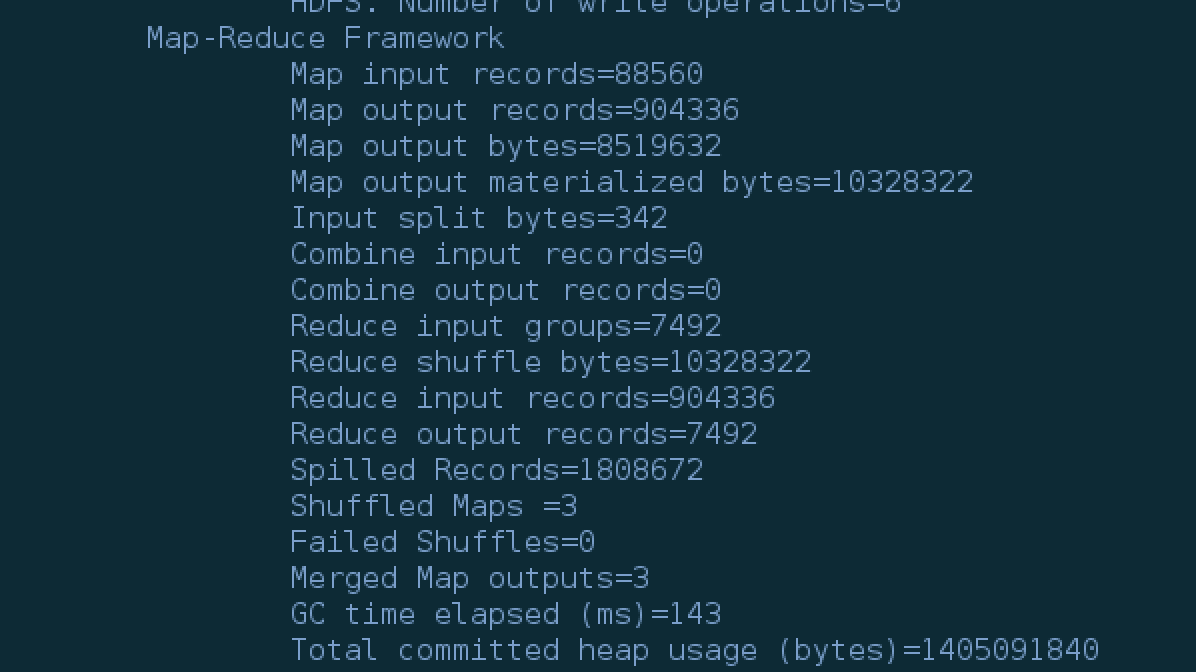
\includegraphics[width=1\textwidth]{images/salidamapreduce.png}
\end{figure}


\chapter{Tutorial de Spark}

\section{Ejemplos de operaciones con RDDs de Spark}

\textbf{Pregunta TS1.1 ¿Cómo hacer para obtener una lista de los elementos al cuadrado?}

Simplemente hay que mapear cada uno de los elementos del RDD ejecutando la función lambda correspondiente.

\begin{lstlisting}[language=Python, caption=]
array = sc.parallelize([1,2,3,4,5,6,7,8,9,10], 2)
rdd = pnumeros.map(lambda e: e*e)
print(rdd.collect())
\end{lstlisting}
\begin{verbatim}
[1, 4, 9, 16, 25, 36, 49, 64, 81, 100]
\end{verbatim}

\vspace{0.8em}

\textbf{Pregunta TS1.2 ¿Cómo filtrar los impares?}

Con la operación \texttt{filter} podemos filtrar a través de la función deseada, en este caso \texttt{e\%2==1}.
\begin{lstlisting}[language=Python, caption=]
rddi = numeros.filter (lambda e: e%2==1)
print (rddi.collect())
\end{lstlisting}
\begin{verbatim}
 [2, 4, 6, 8, 10]   
\end{verbatim}

\vspace{0.8em}

\textbf{Pregunta TS1.3 ¿Tiene sentido esta operación? ¿Si se repite se obtiene siempre el mismo resultado?}

\begin{lstlisting}[language=Python, caption=]
#Tiene sentido esta operacion?
numeros = sc.parallelize([1,2,3,4,5])
print (numeros.reduce(lambda elem1,elem2: elem1-elem2))
numeros = sc.parallelize([1,2,4,3,5])
print (numeros.reduce(lambda elem1,elem2: elem1-elem2))
\end{lstlisting}
\begin{verbatim}
5
3
\end{verbatim}
No tiene sentido ya que \texttt{reduce} es una función monoidal que asume que la función es conmutativa y asociativa, lo que significa que el orden de aplicación a los elementos no está garantizado. Y la función elem1$-$elem2 no es ni asociativa ni conmutativa.

\vspace{0.8em}

\textbf{Pregunta TS1.4 ¿Cómo lo ordenarías para que primero aparezcan los impares y luego los pares?}

Partiendo de las operaciones anteriores podemos filtrar los impares y los pares y con una simple \texttt{union} podemos devolverlo en un RDD único.

\begin{lstlisting}[language=Python, caption=]
numeros = sc.parallelize([5,3,2,1,4])
rdd = numeros.filter(lambda e: e%2==1).union(numeros.filter(lambda e: e%2==0))
rdd.collect()
\end{lstlisting}
\begin{verbatim}
[3, 1, 5, 2, 4]
\end{verbatim}

\vspace{0.8em}

\textbf{Pregunta TS1.5 ¿Cuántos elementos tiene cada RDD? ¿Cuál tiene más?}

Para cada ejemplo se incluye en la salida el número de elementos para cada RDD:

\begin{lstlisting}[language=Python, caption=Ejemplo 1 TS1.5]
palabras = sc.parallelize(['HOLA', 'Que', 'TAL', 'Bien'])
pal_minus = palabras.map(lambda elemento: elemento.lower())
print (pal_minus.collect())
print ("RDD size: ", pal_minus.count())
\end{lstlisting}

\begin{verbatim}
    ['hola', 'que', 'tal', 'bien']
    RDD size:  4
\end{verbatim}

\begin{lstlisting}[language=Python, caption=Ejemplo 2 TS1.5]
palabras = sc.parallelize(['HOLA', 'Que', 'TAL', 'Bien'])
pal_long = palabras.map(lambda elemento: len(elemento))
print (pal_long.collect())
print ("RDD size: ", pal_long.count())
\end{lstlisting}

\begin{verbatim}
    [4, 3, 3, 4]
    RDD size:  2
\end{verbatim}

\begin{lstlisting}[language=Python, caption=Ejemplo 3 TS1.5]
log = sc.parallelize(['E: e21', 'W: w12', 'W: w13', 'E: e45'])
errors = log.filter(lambda elemento: elemento[0]=='E')
print (errors.collect())
print ("RDD size: ", errors.count())
\end{lstlisting}

\begin{verbatim}
    ['E: e21', 'E: e45']
    RDD size:  2
\end{verbatim}

\begin{lstlisting}[language=Python, caption=Ejemplo 4 TS1.5]
lineas = sc.parallelize(['', 'a', 'a b', 'a b c'])
palabras = lineas.flatMap(lambda elemento: elemento.split())
print (palabras.collect())
print ("RDD size: ", palabras.count())
\end{lstlisting}

\begin{verbatim}
    ['a', 'a', 'b', 'a', 'b', 'c']
    RDD size:  6
\end{verbatim}

\begin{lstlisting}[language=Python, caption=Ejemplo 5 TS1.5]
lineas = sc.parallelize(['', 'a', 'a b', 'a b c'])
palabras_flat = lineas.flatMap(lambda elemento: elemento.split())
palabras_map = lineas.map(lambda elemento: elemento.split())
print (palabras_flat.collect())
print (palabras_map.collect())
print ("RDD size palabras_flat: ", palabras_flat.count())
print ("RDD size palabras_map: ", palabras_map.count())
\end{lstlisting}

\begin{verbatim}
['a', 'a', 'b', 'a', 'b', 'c']
[[], ['a'], ['a', 'b'], ['a', 'b', 'c']]
RDD size palabras_flat:  6
RDD size palabras_map:  4
\end{verbatim}

Como podemos comprobar los RDDs de mayor tamaño son \texttt{palabras\_flat} y \texttt{palabras} ya que son los que utilizan la operación \texttt{flatMap}. Como se explica en la pregunta TS2.1, el tamaño del RDD resultante varía dependiendo de la operación. En este caso, al utilizar \texttt{split} para cada elemento se genera un RDD de matrices de palabras, es decir, un resultado anidado que finalmente se aplana y se obtienen los elementos en una única lista.

\vspace{0.8em}

\textbf{Pregunta TS1.6 ¿De qué tipo son los elementos del rdd palabras\_map? ¿Por qué palabras\_map tiene el primer elemento vacío?}

Los elementos resultantes de \texttt{palabras\_flat} son de tipo RDD, al obtenerlos mediante \texttt{collect} se obtienen como elementos de tipo \textit{list}.

Por su parte, \texttt{palabras\_map} tiene el primer elemento vacío porque aplica la operación \texttt{map} a cada uno de los elementos del RDD original, sin cambiar ni aplanar nada más en la salida, a diferencia de \texttt{palabras\_flat}, obteniendo un RDD nuevo del mismo tamaño que el original.

\vspace{0.8em}

\textbf{Pregunta TS1.7. Prueba la transformación distinct si lo aplicamos a cadenas.}

Se puede comprobar que \texttt{distinct} devuelve los elementos únicos de la entrada de partida.

\begin{lstlisting}[language=Python, caption=]
log = sc.parallelize(['E: e21', 'I: i11', 'W: w12', 'I: i11', 'W: w13', 'E: e45'])
infos = log.distinct()
print (infos.collect())
\end{lstlisting}
\begin{verbatim}
    ['I: i11', 'W: w12', 'W: w13', 'E: e45', 'E: e21']
\end{verbatim}
%Duda del notebook! (por que hay una celda ahi que no tiene que ver con la pregunta?)
\vspace{0.8em}

\textbf{Pregunta TS1.8 ¿Cómo se podría obtener la misma salida pero utilizando una sola transformación y sin realizar la unión?}

Dado el código de partida siguiente:

\begin{lstlisting}[language=Python, caption=]
log = sc.parallelize(['E: e21', 'I: i11', 'W: w12', 'I: i11', 'W: w13', 'E: e45'])
infos = log.filter(lambda elemento: elemento[0]=='I')
errors = log.filter(lambda elemento: elemento[0]=='E')
inferr = infos.union(errors)
print (inferr.collect())
\end{lstlisting}
\begin{verbatim}
    ['I: i11', 'I: i11', 'E: e21', 'E: e45']
\end{verbatim}

Se puede modificar la función lambda para que filtre para ambos caracteres de la siguiente manera:

\begin{lstlisting}[language=Python, caption=]
log = sc.parallelize(['E: e21', 'I: i11', 'W: w12', 'I: i11', 'W: w13', 'E: e45'])
infos = log.filter(lambda elemento: (elemento[0]=='I' or elemento[0]== 'E'))
print (infos.collect())
\end{lstlisting}
\begin{verbatim}
    ['E: e21', 'I: i11', 'I: i11', 'E: e45']
\end{verbatim}

De esta manera obtenemos el mismo resultado final.

\vspace{0.8em}

\textbf{Pregunta TS1.9 ¿Cómo explica el funcionamiento de las celdas anteriores?}

%\colorbox{yellow}{A qué celdas se refiereeee??? xddd}

\begin{lstlisting}[language=Python, caption=]
r = sc.parallelize([('A', 1),('C', 4),('A', 1),('B', 1),('B', 4)])
rr1 = r.reduceByKey(lambda v1,v2:v1+v2)
print (rr1.collect())
rr2 = rr1.reduceByKey(lambda v1,v2:v1)
print (rr2.collect())
\end{lstlisting}
\begin{verbatim}
    [('C', 4), ('A', 2), ('B', 5)]
    [('C', 4), ('A', 2), ('B', 5)]
\end{verbatim}
Una vez que se ha aplicado la operación $+$ sobre los valores de las claves comunes, todos los elementos del rdd tienen claves distintas. Por tanto, al aplicar el \texttt{reduceByKey} no se realiza ninguna operación sobre el RDD.

\vspace{0.8em}

\textbf{Pregunta TS1.10 Borra la salida y cambia las particiones en parallelize ¿Qué sucede?}

\begin{lstlisting}[language=Python, caption=]
%rm -rf salida
numeros = sc.parallelize(range(0,1000),10)
numeros.saveAsTextFile('salida')
%ls -la salida/*

n2 = sc.textFile('salida').map(lambda a:int(a))
print(n2.reduce(lambda v1,v2: v1 + v2))
\end{lstlisting}
\begin{verbatim}
-rw-r--r-- 1 root root 290 Oct  6 11:40 salida/part-00000
-rw-r--r-- 1 root root 400 Oct  6 11:40 salida/part-00001
-rw-r--r-- 1 root root 400 Oct  6 11:40 salida/part-00002
-rw-r--r-- 1 root root 400 Oct  6 11:40 salida/part-00003
-rw-r--r-- 1 root root 400 Oct  6 11:40 salida/part-00004
-rw-r--r-- 1 root root 400 Oct  6 11:40 salida/part-00005
-rw-r--r-- 1 root root 400 Oct  6 11:40 salida/part-00006
-rw-r--r-- 1 root root 400 Oct  6 11:40 salida/part-00007
-rw-r--r-- 1 root root 400 Oct  6 11:40 salida/part-00008
-rw-r--r-- 1 root root 400 Oct  6 11:40 salida/part-00009
-rw-r--r-- 1 root root   0 Oct  6 11:40 salida/_SUCCESS
499500
\end{verbatim}

Al particionar los datos en 10 partes, el resultado se escribe en 10 ficheros distintos con tamaño máximo igual a 400 bytes.

\section{El Quijote}

\textbf{Pregunta TS2.1 Explica la utilidad de cada transformación y detalle para cada una de ellas si cambia el número de elementos en el RDD resultante. Es decir si el RDD de partida tiene N elementos, y el de salida M elementos, indica si N>M, N=M o N<M.}
\begin{itemize}
    \item \texttt{map}: aplica una función a cada elemento del RDD transformando un RDD de longitud $N$ en otro de longitud $N$.
    \item \texttt{flatmap}: aplica una función a cada elemento de un RDD y devuelve el resultado aplanado. En términos generales, transforma un RDD de longitud $N$ en una colección de $N$ colecciones, que luego aplana en un solo RDD. De esta manera se obtienen diferente número de elementos de entrada y de salida. Dependiendo de la operación, puede devolver un $M$ que puede ser mayor, menor o igual a $N$.
    \item \texttt{filter}: operación que devuelve un nuevo RDD que contiene elementos que satisfacen un predicado (\textit{boolean}), mapeando uno a uno. Por tanto $M=N$.
    \item \texttt{distinct}: dado un RDD, obtiene un nuevo RDD con los elementos únicos de su entrada, por lo que se tiene que satisfacer que $M \leq N$ estrictamente.
    \item \texttt{sample}: en este caso se obtiene un subset aleatorio de un RDD dado. Dependiendo de si se da con reemplazamiento o no, se puede obtener que $M \leq N$ o $M>N$.
    \item \texttt{union}: concatena dos RDDs en uno, luego el resultado final será $M=N_1 + N_2$, dados $N_1$ y $N_2$ el tamaño de las entradas respectivamente.
\end{itemize}

\vspace{0.8em}

\textbf{Pregunta TS2.2 Explica el funcionamiento de cada acción anterior.}
\textbf{Implementa la opción count de otra manera:}
\begin{itemize}
    \item \textbf{Utilizando transformaciones Map y Reduce.}
    
    Para ello se requiere hacer un mapeo por cada línea con \texttt{charsPerLine} y después se aplica la operación suma con un \texttt{reduce} como se puede ver a continuación.
    
    \begin{lstlisting}[language=Python, caption=]
charsPerLine = quijote.map(lambda s: len(s))

numLines = quijote.count()
numChars = charsPerLine.reduce(lambda a,b: a+b) # also charsPerLine.sum()
sortedWordsByLength = allWordsNoArticles.takeOrdered(20, key=lambda x: -len(x))
numLines, numChars, sortedWordsByLength
    \end{lstlisting}
    La salida se muestra a continuación, siendo 5534 el número de líneas y 305678 el número de caracteres.
    \begin{verbatim}
(5534,
 305678,
 ['procuremos.Levántate,',
  'estrechísimamente,',
  'Pintiquiniestra,',
  'entretenimiento,',
  'maravillosamente',
  'descansadamente;',
  'desenfadadamente',
  'quebrantamientos',
  'quebrantamiento,',
  'alternativamente',
  'encantamientos,',
  'Placerdemivida,',
  'encantamientos;',
  'malbaratándolas',
  'regocijadamente',
  'consentimiento,',
  'desaconsejaban,',
  'acontecimiento.',
  'agradeciéndoles',
  'encantamientos,'])
    \end{verbatim}
    
    \item \textbf{Utilizando solo \texttt{reduce} en caso de que sea posible.}
    La única manera para poder realizar una operación atómica con \texttt{reduce} es a través de la creación de una función propia que sume líneas y otra para sumar caracteres.
    
\begin{lstlisting}[language=Python, caption=]
quijote = sc.textFile("quijote.txt")
def count_lines(a, b):
  if isinstance(a, str):
    a = 1
  if isinstance(b, str):
    b = 1
  return a + b
quijote.reduce(count_lines)
\end{lstlisting}
\begin{verbatim}
5534
\end{verbatim}

\begin{lstlisting}[language=Python, caption=]
def count_chars(a,b):
  if isinstance(a, str):
    if isinstance(b, str):
      return len(a) + len(b)
    else:
      return len(a) + b 
  else:
    if isinstance(b, str):
      return a + len(b)
    else:
      return a + b
  
quijote.reduce(count_chars)
\end{lstlisting}
\begin{verbatim}
305678
\end{verbatim}
    
\end{itemize}



\vspace{0.8em}

\textbf{Pregunta TS2.3 Explica el propósito de cada una de las operaciones anteriores.}

Las operaciones \textit{key-value} con RDDs son un tipo especial de RDDs donde cada elemento es una tupla clave (K) valor (V). 

En esta parte se utiliza el fichero \texttt{quijote.txt} original y se descarga otro que es más largo. Las palabras se filtran y se guardan en \texttt{allWords} (56521 palabras) y \texttt{allWords2} (197777 palabras) respectivamente.

\begin{lstlisting}[language=Python, caption=]
words = allWords.map(lambda e: (e,1))
words2 = allWords2.map(lambda e: (e,1))

words.take(10)
\end{lstlisting}
\begin{verbatim}
[('el', 1),
 ('ingenioso', 1),
 ('hidalgo', 1),
 ('don', 1),
 ('quijote', 1),
 ('de', 1),
 ('la', 1),
 ('mancha', 1),
 ('miguel', 1),
 ('de', 1)]
\end{verbatim}

En este caso se realiza una operación \textit{K-V}, con $(V)=1$ para cada una de las palabras.

\begin{lstlisting}[language=Python, caption=]
frequencies = words.reduceByKey(lambda a,b: a+b)
frequencies2 = words2.reduceByKey(lambda a,b: a+b)
frequencies.takeOrdered(10, key=lambda a: -a[1])
\end{lstlisting}
\begin{verbatim}
[('que', 3032),
 ('de', 2809),
 ('y', 2573),
 ('a', 1426),
 ('la', 1423),
 ('el', 1232),
 ('en', 1155),
 ('no', 903),
 ('se', 753),
 ('los', 696)]
\end{verbatim}

En este ejemplo se ha hecho uso de \texttt{reduceByKey}, operación que combina los valores de cada clave utilizando \texttt{reduce} asociativo y conmutativo. De esta manera, se cuenta con una lambda que suma la frecuencia de cada una de las palabras almacenándolo en una tupla \textit{K-V}, mostrándolo en orden descendente. 


%La salida se dividirá con las particiones numPartitions, o el nivel de paralelismo por defecto si no se especifica numPartitions. El particionador por defecto es hash-partición.



\begin{lstlisting}[language=Python, caption=]
res = words.groupByKey().takeOrdered(10, key=lambda a: -len(a))
res # To see the content, res[i][1].data
\end{lstlisting}
\begin{verbatim}
[('el', <pyspark.resultiterable.ResultIterable at 0x7f65597530d0>),
 ('hidalgo', <pyspark.resultiterable.ResultIterable at 0x7f65599c7cd0>),
 ('don', <pyspark.resultiterable.ResultIterable at 0x7f65599ac510>),
 ('mancha', <pyspark.resultiterable.ResultIterable at 0x7f655974f950>),
 ('saavedra', <pyspark.resultiterable.ResultIterable at 0x7f655974fb50>),
 ('que', <pyspark.resultiterable.ResultIterable at 0x7f655974f910>),
 ('condición', <pyspark.resultiterable.ResultIterable at 0x7f655974f090>),
 ('y', <pyspark.resultiterable.ResultIterable at 0x7f655974f150>),
 ('del', <pyspark.resultiterable.ResultIterable at 0x7f655974f1d0>),
 ('d', <pyspark.resultiterable.ResultIterable at 0x7f655974fb10>)]
\end{verbatim}

En este caso se ha hecho uso de \texttt{groupByKey}, operación que agrupa los valores de cada clave en el RDD en una única secuencia iterable. En este caso, se ordenan de menor a mayor. El contenido de esta salida se puede ver como en el siguiente ejemplo para el caso de la clave ``mancha'':

\begin{lstlisting}[language=Python, caption=]
res[3][1].data
\end{lstlisting}
\begin{verbatim}
[1, 1, 1, 1, 1, 1, 1, 1, 1, 1, 1, 1, 1, 1, 1, 1, 1, 1, 1, 1, 1, 1, 1, 1, 1, 1]
\end{verbatim}

En definitiva, 26

\begin{lstlisting}[language=Python, caption=]
joinFreq = frequencies.join(frequencies2)
joinFreq.take(10)
\end{lstlisting}
\begin{verbatim}
[('el', (1232, 4394)),
 ('hidalgo', (14, 42)),
 ('don', (370, 1606)),
 ('mancha', (26, 101)),
 ('saavedra', (1, 1)),
 ('que', (3032, 10040)),
 ('y', (2573, 9650)),
 ('del', (415, 1344)),
 ('en', (1155, 4223)),
 ('cuyo', (11, 35))]
\end{verbatim}

En este caso, se relación una combinación de los RDD's \texttt{frequencies} y \texttt{frequencies2} a partir de la operación \texttt{join}, de manera que se agrupan los valores de las claves comunes.

\begin{lstlisting}[language=Python, caption=]
joinFreq.map(lambda e: (e[0], (e[1][0] - e[1][1])/(e[1][0] + e[1][1]))).takeOrdered(10, lambda v: -v[1]), joinFreq.map(lambda e: (e[0], (e[1][0] - e[1][1])/(e[1][0] + e[1][1]))).takeOrdered(10, lambda v: +v[1])
\end{lstlisting}
\begin{verbatim}
([('pieza', 0.8),
  ('corral', 0.8),
  ('rodela', 0.7777777777777778),
  ('curar', 0.75),
  ('valle', 0.75),
  ('entierro', 0.75),
  ('oh', 0.7142857142857143),
  ('licor', 0.7142857142857143),
  ('difunto', 0.7142857142857143),
  ('pago', 0.6666666666666666)],
 [('teresa', -0.9767441860465116),
  ('roque', -0.96),
  ('paje', -0.9565217391304348),
  ('duque', -0.9565217391304348),
  ('blanca', -0.9565217391304348),
  ('gobernador', -0.9503105590062112),
  ('diego', -0.9459459459459459),
  ('tarde', -0.9428571428571428),
  ('mesmo', -0.9381443298969072),
  ('letras', -0.9354838709677419)])
\end{verbatim}

Esta operación asigna una distancia entre $(-1,1)$ a las palabras de los conjuntos de datos \texttt{frequencies} y \texttt{frequencies2}. Se asignan valores próximos a 1 a aquellas palabras que aparecen un mayor número de veces en \texttt{frequencies} y un valor próximo a -1 a aquellas palabras que aparecen un mayor número de veces en \texttt{frequencies2}. Por el contrario, las palabras que se aproximan a 0 son aquellas que aparecen el mismo número de veces en ambos conjuntos. 

De esta manera, el primer conjunto muestra las palabras que aparecen con más frecuencia en \texttt{frequencies} y en el segundo conjunto muestra aquellas palabras que aparecen con más frecuencia en \texttt{frequencies2}.

\vspace{0.8em}

\textbf{Pregunta TS2.4 ¿Cómo puede implementarse la frecuencia con groupByKey y transformaciones?}

\begin{lstlisting}[language=Python, caption=]
words.groupByKey().map(lambda e:(e[0], sum(e[1]))).takeOrdered(10, key=lambda a: -a[1])
\end{lstlisting}
\begin{verbatim}
[('que', 3032),
 ('de', 2809),
 ('y', 2573),
 ('a', 1426),
 ('la', 1423),
 ('el', 1232),
 ('en', 1155),
 ('no', 903),
 ('se', 753),
 ('los', 696)]
\end{verbatim}

\vspace{0.8em}

\textbf{Pregunta TS2.5 ¿Cuál de las dos siguientes celdas es más eficiente? Justifique la respuesta.}

\begin{lstlisting}[language=Python, caption=]
joinFreq.map(lambda e: (e[0], (e[1][0] - e[1][1])/(e[1][0] + e[1][1]))).takeOrdered(10, lambda v: -v[1]), joinFreq.map(lambda e: (e[0], (e[1][0] - e[1][1])/(e[1][0] + e[1][1]))).takeOrdered(10, lambda v: +v[1])
\end{lstlisting}

\begin{lstlisting}[language=Python, caption=]
result = joinFreq.map(lambda e: (e[0], (e[1][0] - e[1][1])/(e[1][0] + e[1][1])))
result.cache()
result.takeOrdered(10, lambda v: -v[1]), result.takeOrdered(10, lambda v: +v[1])
\end{lstlisting}


Es más eficiente la segunda celda ya que al guardar los resultados en cache, se acelera el proceso de acceder a los datos al realizar la operación \texttt{takeOrdered}.
\vspace{0.8em}

\textbf{Pregunta TS2.6 Antes de guardar el fichero, utilice coalesce con diferentes valores ¿Cuál es la diferencia?}

Para poder explicar esta pregunta debemos primer tener clara la diferencia entre \texttt{coalesce} y \texttt{repartition}:

\begin{itemize}
    \item \texttt{coalesce}: se utiliza para reducir el número de particiones, tratando de minimizar el movimiento de datos evitando la red aleatoria. De esta manera, crea particiones de tamaño desigual.
    \item \texttt{repartition}: se utiliza para reducir o disminuir el número de particiones, activando una red aleatoria que puede aumentar el movimiento de datos. De esta manera, crea particiones de igual tamaño.
\end{itemize}


En local las particiones son equivalentes, pero en un cluster son distintas, obteniendo un fichero por cada partición.

Probando con diferentes particiones:

\begin{lstlisting}[language=Python, caption=]
rdd = result.repartition(numPartitions=3)
rdd
\end{lstlisting}

2 ejecuciones:
\begin{verbatim}
MapPartitionsRDD[269] at coalesce at NativeMethodAccessorImpl.java:0
\end{verbatim}

\begin{verbatim}
MapPartitionsRDD[274] at coalesce at NativeMethodAccessorImpl.java:0
\end{verbatim}

\begin{lstlisting}[language=Python, caption=]
rdd = result.repartition(numPartitions=3)
rdd.getNumPartitions()
\end{lstlisting}
\begin{verbatim}
3
\end{verbatim}

\begin{lstlisting}[language=Python, caption=]
rdd = result.repartition(numPartitions=8)
rdd.getNumPartitions()
\end{lstlisting}
\begin{verbatim}
8
\end{verbatim}



\begin{lstlisting}[language=Python, caption=]
rdd = result.coalesce(numPartitions=3)
rdd
\end{lstlisting}
2 ejecuciones:

\begin{verbatim}
CoalescedRDD[279] at coalesce at NativeMethodAccessorImpl.java:0
\end{verbatim}

\begin{verbatim}
CoalescedRDD[280] at coalesce at NativeMethodAccessorImpl.java:0
\end{verbatim}

\begin{lstlisting}[language=Python, caption=]
rdd = result.coalesce(numPartitions=3)
rdd.getNumPartitions()
\end{lstlisting}
\begin{verbatim}
2
\end{verbatim}

\begin{lstlisting}[language=Python, caption=]
rdd = result.coalesce(numPartitions=8)
rdd.getNumPartitions()
\end{lstlisting}
\begin{verbatim}
2
\end{verbatim}


%\colorbox{yellow}{El algoritmo de repartición se usa para aumentar o disminuir las particiones RDD, mientras que coalesce evita el movimiento de datos tratando de equilibrar los datos dentro de cada máquina.}

\chapter{Ejercicios opcionales}

Toda la información relativa al código implementado, los conjuntos de datos utilizados y la salida proporcionada por cada aplicación se encuentran en los directorios \textbf{QualityDesc/} y \textbf{ClubAgeDesc/} de la entrega.


\section{Calidad del aire}

Este ejercicio implementa una aplicación que calcula estadísticas descriptivas de un conjunto de datos de la calidad del aire \url{http://datosabiertos.jcyl.es/web/jcyl/set/es/mediciones/calidad_aire_historico/1284212629698}. En particular, la aplicación devuelve la media, el valor mínimo y el valor máximo de la calidad del aire por provincia de España. Se ha implementado la clase \texttt{QualityDesc} en Java y los métodos \texttt{QualityDescMapper} y \texttt{QualityDescReducer}, disponible en el archivo \textbf{QualityDesc.java} entregado. 
\begin{lstlisting}[language=Java, caption=]
public static class QualityDescMapper extends Mapper<Object, Text, Text, DoubleWritable> {

	private static final String SEPARATOR = ";";

	public void map(Object key, Text value, Context context) throws IOException, InterruptedException {
		final String[] values = value.toString().split(SEPARATOR);


		final String co = format(values[1]);
		final String province = format(values[8]);

		if (NumberUtils.isNumber(co.toString())) {
			context.write(new Text(province), new DoubleWritable(NumberUtils.toDouble(co)));
		}
	}

	private String format(String value) {
		return value.trim();
	}
}
\end{lstlisting}
\begin{lstlisting}[language=Java, caption=]
public static class QualityDescReducer extends Reducer<Text, DoubleWritable, Text, Text> {

		private final DecimalFormat decimalFormat = new DecimalFormat("#.##");

		public void reduce(Text key, Iterable<DoubleWritable> coValues, Context context) throws IOException, InterruptedException {
			int measures = 0;
			double totalCo = 0.0f;
			double min = Double.POSITIVE_INFINITY;
			double max = Double.NEGATIVE_INFINITY;

			for (DoubleWritable coValue : coValues) {
				double val = coValue.get();
				totalCo += val;
				measures++;

				if (min > val) {
					min = val;
				}
				if (max < val) {
					max = val;				
				}
			}
			

			if (measures > 0) {
				context.write(key, new Text(decimalFormat.format(totalCo / measures) + ' ' + decimalFormat.format(min) + ' ' + decimalFormat.format(max)));
			}
		}
	}
\end{lstlisting}

\begin{lstlisting}[language=Java, caption=]
public static void main(String[] args) throws Exception {
    Configuration conf = new Configuration();

    /*String[] otherArgs = new GenericOptionsParser(conf, args).getRemainingArgs();
    if (otherArgs.length != 2) {
      System.err.println("Usage: wordcount <in> <out>");
      System.exit(2);
    }*/

    @SuppressWarnings("deprecation")
    Job job = new Job(conf, "qualitydesc");
		job.setJarByClass(QualityDesc.class);
		job.setInputFormatClass(TextInputFormat.class);
		job.setOutputFormatClass(TextOutputFormat.class);

		job.setMapperClass(QualityDescMapper.class);
		job.setReducerClass(QualityDescReducer.class);

		job.setMapOutputKeyClass(Text.class);
		job.setMapOutputValueClass(DoubleWritable.class);
		job.setOutputKeyClass(Text.class);
		job.setOutputValueClass(Text.class);

    FileInputFormat.addInputPath(job, new Path(args[0]));
    FileOutputFormat.setOutputPath(job, new Path(args[1]));

    System.exit(job.waitForCompletion(true) ? 0 : 1);
  }
}
\end{lstlisting}

Tras compilar la aplicación y ejecutarla en Hadoop para el conjunto de datos proporcionado se ha obtenido la siguiente salida (\textbf{salida\_quality\_desc.txt}):
\begin{verbatim}
Avila	0,96 0,1 8,6
Burgos	0,76 0 8,7
León	0,89 0 25,1
Palencia	1,13 0,1 12,1
Salamanca	1,32 0,1 11,1
Segovia	0,92 0,1 5
Soria	0,35 0,1 1
Valladolid	0,51 0 6,4
Zamora	0,8 0,1 3,6
\end{verbatim}

\section{Edad de los jugadores de un Club}
Este ejercicio implementa una aplicación que calcula un resumen numérico de las edades medias, máximas y mínimas de los jugadores de distintos club de Futbol. El dataset utilizado para realizar las pruebas se ha obtenido de \url{https://www.kaggle.com/karangadiya/fifa19/version/4} y previamente a utilizarlo en Hadoop se ha realizado una limpieza utilizando los siguientes comandos de Python:
\begin{lstlisting}[language=Python, caption=]
import pandas as pd
col_list = ['Name','Age','Club']
df = pd.read_csv("original_clubagedata.csv", usecols=col_list)
df.dropna(inplace=True)
df.to_csv('clubagedata.csv', sep=',',header=None, index=False)
\end{lstlisting}

La aplicación devuelve la media, el valor mínimo y el valor máximo de la edades de los jugadores por club. Se ha implementado la clase \texttt{ClubAgeDesc} en Java y los métodos \texttt{ClubAgeDescMapper} y \texttt{ClubAgeDescReducer}, disponible en el archivo \textbf{ClubAgeDesc.java} entregado. 
Se ha modificado el nombre de la clase y el nombre de los métodos y, en particular, para el método Map se han modificado únicamente los índices de interés y el separador.
\begin{lstlisting}[language=Java, caption=]
public static class ClubAgeDescMapper extends Mapper<Object, Text, Text, DoubleWritable> {

    private static final String SEPARATOR = ",";
    
    public void map(Object key, Text value, Context context) throws IOException, InterruptedException {
    	final String[] values = value.toString().split(SEPARATOR);
    
    	
    	final String age = format(values[1]);
    	final String club = format(values[2]);
    
    	if (NumberUtils.isNumber(age.toString())) {
    		context.write(new Text(club), new DoubleWritable(NumberUtils.toDouble(age)));
    	}
    }
    
    private String format(String value) {
    	return value.trim();
    }
}
\end{lstlisting}

La salida devuelta por Hadoop se encuentra en el fichero \textbf{salida\_clubage\_desc.txt} y una muestra de la salida devuelta por Hadoop se muestra a continuación:
\begin{verbatim}
MKE Ankaragücü	28,59 20 36
MSV Duisburg	24,88 18 35
Macclesfield Town	25,46 19 37
Malmö FF	25,41 18 35
Manchester City	23,91 17 35
Manchester United	24,76 17 35
Mansfield Town	24,46 17 36
Medipol Başakşehir FK	27,46 18 37
Melbourne City FC	25,36 18 37
Melbourne Victory	25,57 18 33
Middlesbrough	25,5 17 39
Miedź Legnica	26,89 17 37
Milan	25 18 35
Millonarios FC	26,57 18 34
Millwall	24,7 18 34
Milton Keynes Dons	24,64 17 34
Minnesota United FC	26,53 19 34
Molde FK	23,77 17 35
Monarcas Morelia	25 18 36
Monterrey	24,69 17 34
Montpellier HSC	24,75 18 40
Montreal Impact	26,14 19 36
Morecambe	25,07 18 39
Moreirense FC	25,48 18 34
Motherwell	24,04 17 31
Málaga CF	25,33 17 34
\end{verbatim}

\end{document}
